\section{Algorithm}
\subsection{Constructing the mapping}\label{subsec:map}
\begin{figure}
	\centering
	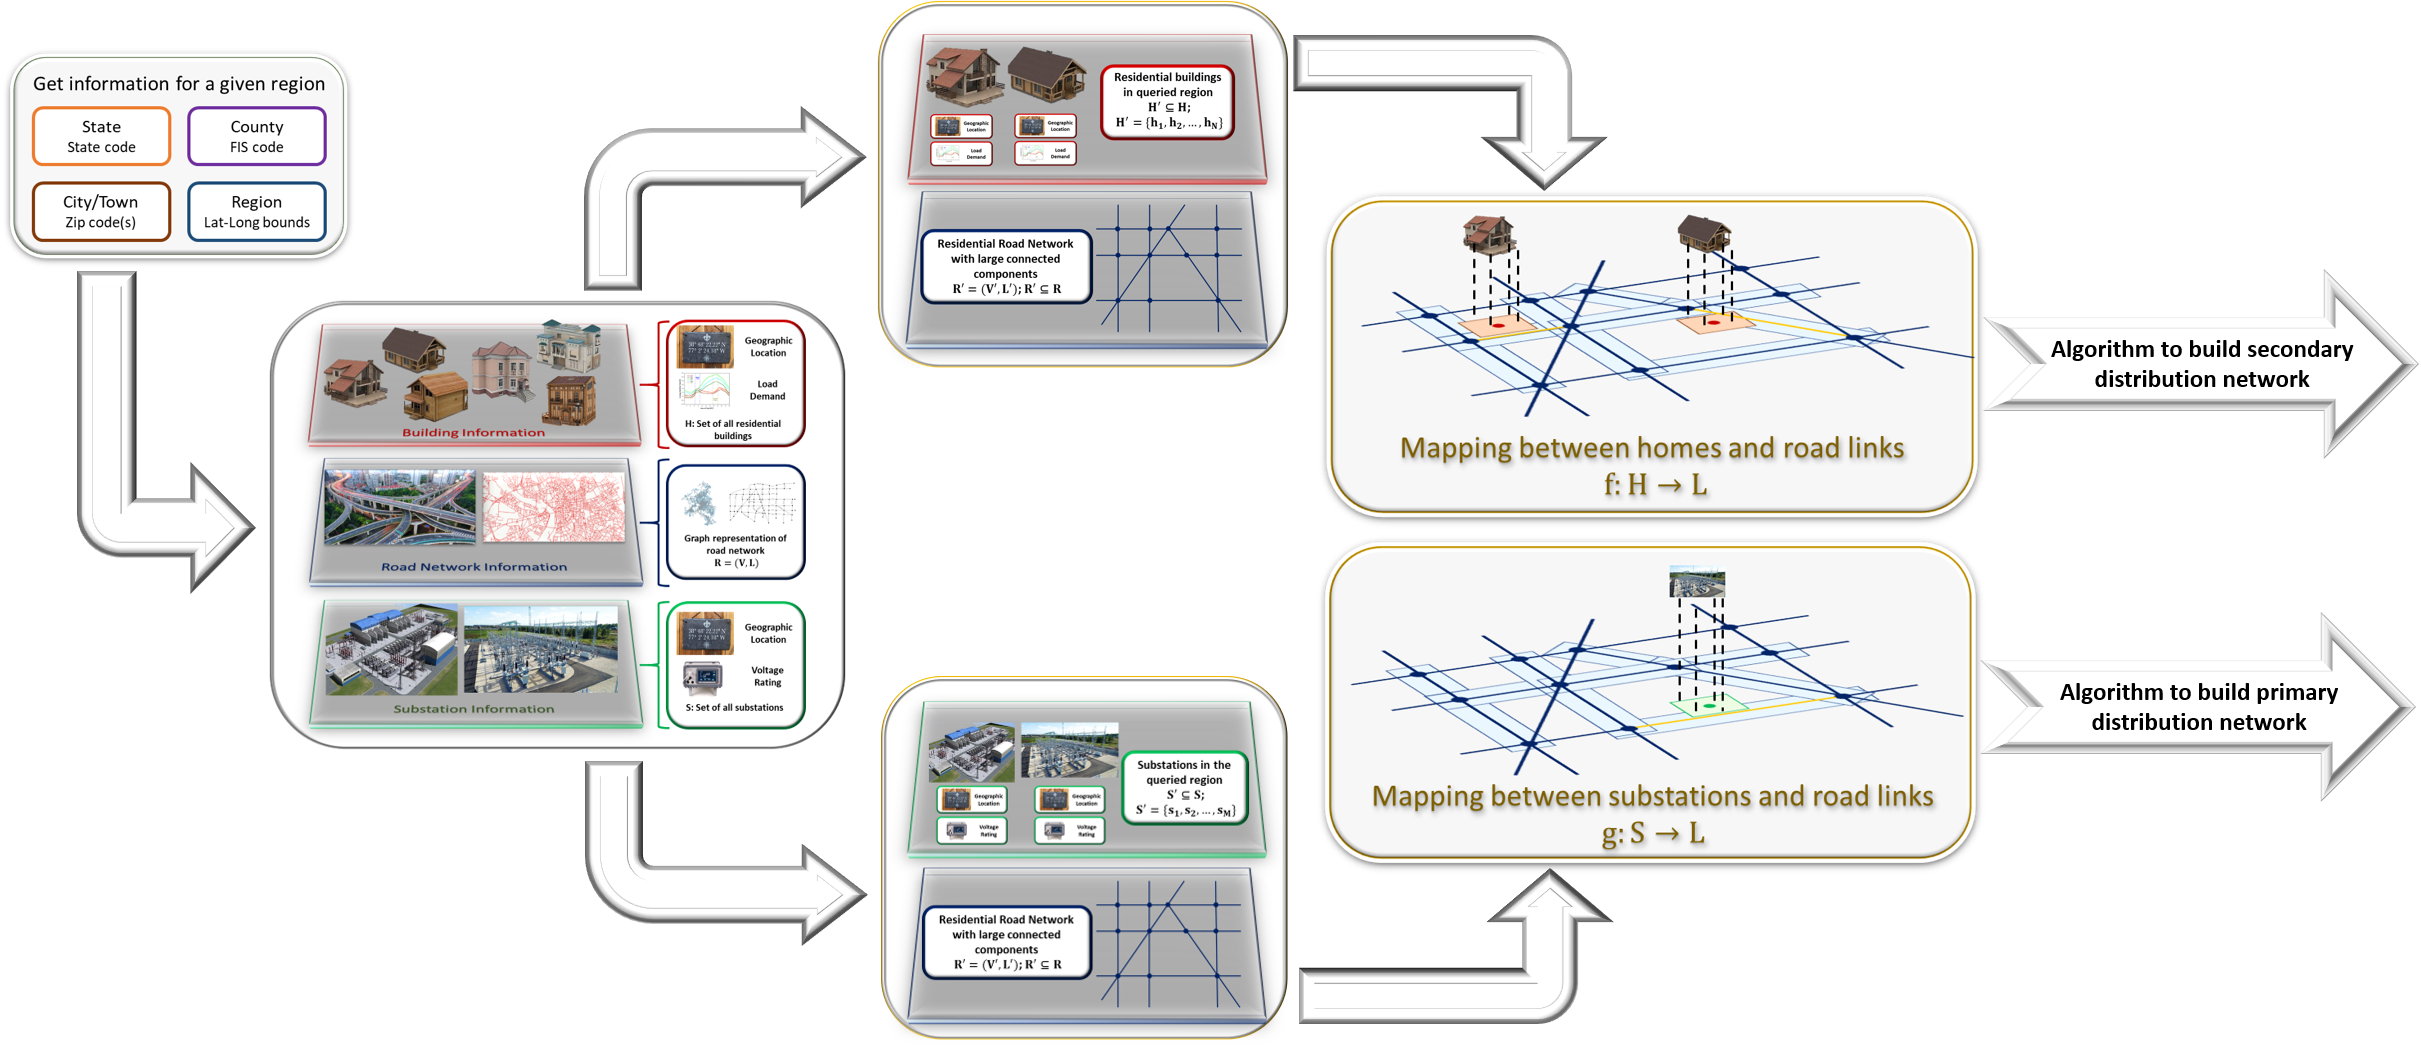
\includegraphics[scale=0.42]{pipeline_1}
	\caption{Flowchart showing the generation of maps between three data sets.}
\end{figure}
\begin{algorithm}[H]
	\caption{Find the nearest link in $\mathsf{L}$ to a given point $\mathbf{p}$.}
	\label{alg:dist}
	\begin{algorithmic}[1]
		\Require Radius for bounding boxes $r$, a mapping $\mathsf{dist}:\mathbb{R}^2\times\mathsf{L}\rightarrow\mathbb{R}^{+}$ such that $\mathsf{dist}(\mathbf{p},\mathbf{l})$ is the shortest distance between point $\mathbf{p}\in\mathbb{R}^2$ and link segment $\mathbf{l}=\mathbf{u}-\mathbf{v}$ for $\mathbf{l}\in\mathsf{L}$ and $\mathbf{u},\mathbf{v}\in\mathbb{R}^2$.
		\For {each link $\mathbf{l}\in\mathsf{L}$}
		\State evaluate bounding box $\mathbf{B_l}$ such that $\mathbf{B_l}=\big\{\mathbf{x}\big|||\mathbf{x}-\mathbf{x_l}||_2\leq r,\forall \mathbf{x_l}=\theta\mathbf{u}+(1-\theta)\mathbf{v},\theta=[0,1]\big\}$.
		\EndFor
		\State Evaluate bounding box $\mathbf{B_p}$ for point $\mathbf{p}$ such that $\mathbf{B_l}=\big\{\mathbf{x}\big|||\mathbf{x}-\mathbf{p}||_2\leq r\big\}$.
		\State Find the bounding boxes $\mathbf{B_{l_1}},\mathbf{B_{l_2}},\cdots,\mathbf{B_{l_m}}$ which intersect with $\mathbf{B_p}$.
		\State Find the link $\mathbf{l^\star}\in\mathsf{L'}$, where $\mathsf{L'}=\{\mathbf{l_1},\mathbf{l_2},\cdots,\mathbf{l_m}\}\subseteq\mathsf{L}$ such that $\mathbf{l^\star}=\argmin_{\mathbf{l}\in\mathsf{L}}\mathsf{dist}(\mathbf{p},\mathbf{l})$.
	\end{algorithmic}
\end{algorithm}
\begin{algorithm}[H]
	\caption{Generate mapping between building and road network data sets.}
	\label{alg:map1}
	\begin{algorithmic}[1]
		\Require Road network graph $\mathsf{R=(\mathsf{V},\mathsf{L})}$, set of residential buildings $\mathsf{H}$, a mapping $\mathsf{dist}:\mathsf{H}\times\mathsf{V}\rightarrow\mathbb{R}^{+}$ such that $\mathsf{dist}(h,v)$ is the Euclidean distance between building $h\in\mathsf{H}$ and road network node $v\in\mathsf{V}$.
		\Initialize :A mapping from road nodes to set of sets of buildings $p:\mathsf{V}\rightarrow\mathcal{H}$ such that $p(v)=\emptyset,\forall v\in\mathsf{V}$
		\For {each building $h\in\mathsf{H}$}
		\State find mapping $f:\mathsf{H}\rightarrow\mathsf{L}$ using Algorithm~\ref{alg:dist} to generate the nearest link $e\in\mathsf{L}$.
		\EndFor
		\For {each link $e=(u,v)\in\mathsf{L}$}
		\State Initialize four sets: $\mathsf{H_{uA}},\mathsf{H_{vA}},\mathsf{H_{uB}},\mathsf{H_{vB}}=\emptyset$.
		\State find the inverse mapping $f^{-1}:\mathsf{L}\rightarrow\mathsf{H}$ which generates the set of buildings $\mathsf{H_e}$ associated with $e$.
		\State find the set of buildings $\mathsf{H_{eA}},\mathsf{H_{eB}}\subseteq\mathsf{H_e}$ with $\mathsf{H_{eA}}\cup\mathsf{H_{eB}}=\mathsf{H_e}$ which are on opposite sides of $e$.
		\For {each building $h\in\mathsf{H_{eA}}$}
		\If {$\mathsf{dist}(h,u)<\mathsf{dist}(h,v)$}
		\State Add this building to set $\mathsf{H_{uA}}$: $\mathsf{H_{uA}}\leftarrow\mathsf{H_{uA}}\cup\{h\}$
		\Else
		\State Add this building to set $\mathsf{H_{vA}}$: $\mathsf{H_{vA}}\leftarrow\mathsf{H_{vA}}\cup\{h\}$
		\EndIf
		\EndFor
		\For {each building $h\in\mathsf{H_{eB}}$}
		\If {$\mathsf{dist}(h,u)<\mathsf{dist}(h,v)$}
		\State Add this building to set $\mathsf{H_{uB}}$: $\mathsf{H_{uB}}\leftarrow\mathsf{H_{uB}}\cup\{h\}$
		\Else
		\State Add this building to set $\mathsf{H_{vB}}$: $\mathsf{H_{vB}}\leftarrow\mathsf{H_{vB}}\cup\{h\}$
		\EndIf
		\EndFor
		\State Add the sets $\mathsf{H_{uA}},\mathsf{H_{uB}}$ to the mapping $p(u)$: $p(u)\leftarrow p(u)\cup\{\mathsf{H_{uA}},\mathsf{H_{uB}}\}$.
		\State Add the sets $\mathsf{H_{vA}},\mathsf{H_{vB}}$ to the mapping $p(v)$: $p(v)\leftarrow p(v)\cup\{\mathsf{H_{vA}},\mathsf{H_{vB}}\}$.
		\EndFor
	\end{algorithmic}
\end{algorithm}

\begin{algorithm}[H]
	\caption{Generate mapping between substations and road network nodes.}
	\label{alg:map2}
	\begin{algorithmic}[1]
		\Require Road network graph $\mathsf{R=(\mathsf{V},\mathsf{L})}$, set of substations $\mathsf{S}$, a mapping $\mathsf{dist}:\mathsf{S}\times\mathsf{V}\rightarrow\mathbb{R}^{+}$ such that $\mathsf{dist}(s,v)$ is the Euclidean distance between substation $s\in\mathsf{S}$ and road network node $v\in\mathsf{V}$, mapping $p:\mathsf{V}\rightarrow\mathcal{H}$ obtained from Algorithm~\ref{alg:map1}, minimum number of road network nodes mapped to a substation $N_{min}$.
		\For {each road network node $v\in\mathsf{V}$}
		\If {$p(v)=\emptyset$}
		\State Remove node $v$ from set of all road network nodes $\mathsf{V}\leftarrow\mathsf{V}\setminus\{v\}$.
		\Else 
		\State Find a mapping $g:\mathsf{V}\rightarrow\mathsf{S}$ which identifies the nearest substation to the road node $v$ such that $g(v)=\argmin_{s\in\mathsf{S}}\mathsf{dist}(s,v)$.
		\EndIf
		\EndFor
		\For {each substation $s\in\mathsf{S}$}
		\State Find inverse mapping $g^{-1}:\mathsf{S}\rightarrow\mathsf{V}$ which generates the set of road network nodes $\mathsf{V_s}$ associated with $s$.
		\If {$|g^{-1}(s)|<N_{min}$}
		\State Remove the substation from set of all substations, $\mathsf{S}\leftarrow\mathsf{S}\setminus\{s\}$
		\EndIf 
		\EndFor
		\State Recompute mapping $g:\mathsf{V}\rightarrow\mathsf{S}$ which identifies the nearest substation to the road node $v$ such that $g(v)=\argmin_{s\in\mathsf{S}}\mathsf{dist}(s,v)$.
	\end{algorithmic}
\end{algorithm}

\begin{figure}[H]
	\centering
	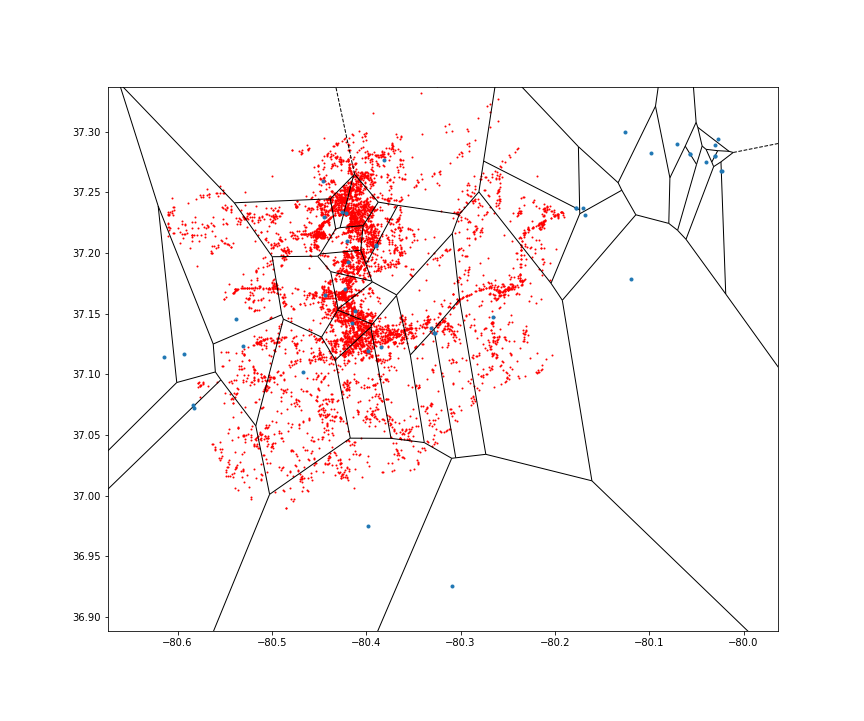
\includegraphics[scale=0.42]{map1}
	\caption{Voronoi regions formed by substations (blue points) and the road nodes (red points) mapped within each region. A number of substations have very road nodes associated with it. Therefore, the Voronoi regions are recomputed after removing the unmapped substations.}
\end{figure}

\begin{figure}[H]
	\centering
	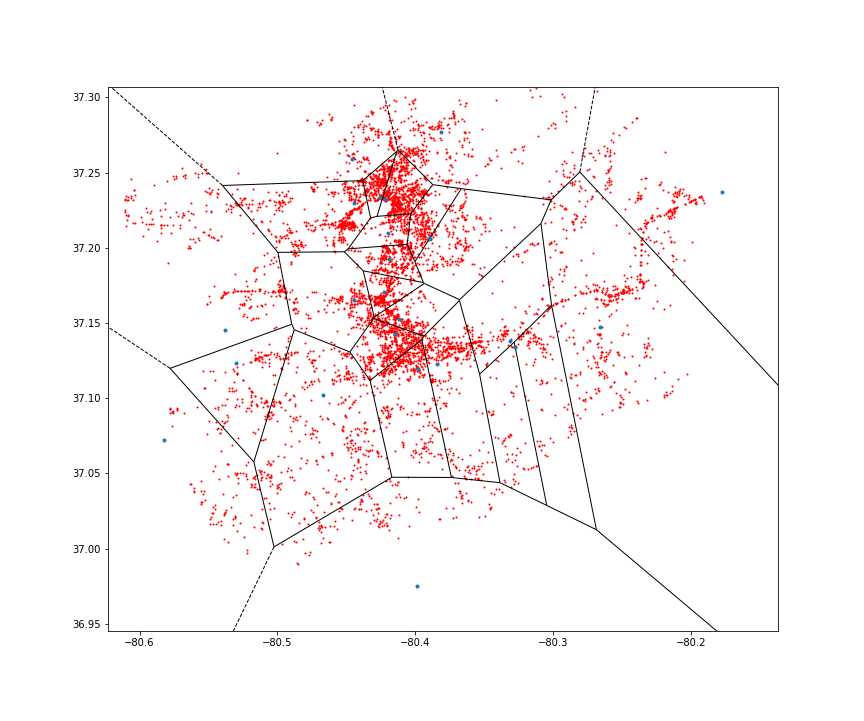
\includegraphics[scale=0.42]{map2}
	\caption{Voronoi regions formed by substations (blue points) and the road nodes (red points) mapped within each region. Almost all the regions are densely distributed by road network nodes. The boundary regions seem to be empty. However, they would be filled by road nodes from the neighboring counties.}
\end{figure}
